% ---
% autor     : Marcelo dos Santos <santos.marcelo@ufabc.edu.br>
% disciplina: Trabalho de Conclusão de Curso (TCC)
% título    : Aplicações da Tecnologia Java para a Internet das Coisas
% curso     : Curso de Especialização em Tecnologias e Sistemas de Informação
%
% ---

\documentclass[
    % -- opções da classe memoir --
    12pt,               % tamanho da fonte
    openright,          % capítulos começam em página ímpar (insere página vazia caso preciso)
    oneside,            % impressão em verso e anverso. Oposto a oneside
    a4paper,            % tamanho do papel
    % -- opções da classe abntex2 --
    chapter=TITLE,      % títulos de capítulos convertidos em letras maiúsculas
    %section=TITLE,     % títulos de seções convertidos em letras maiúsculas
    %subsection=TITLE,  % títulos de subseções convertidos em letras maiúsculas
    %subsubsection=TITLE,% títulos de subsubseções convertidos em letras maiúsculas
    sumario=tradicional,
    %sumario=abnt-6027-2012,
    % -- opções do pacote babel --
    english,            % idioma adicional para hifenização
    french,             % idioma adicional para hifenização
    spanish,            % idioma adicional para hifenização
    brazil              % o último idioma é o principal do documento
]{abntex2}

% ---
% PACOTES BÁSICOS
% ---
\usepackage{times}          % Usa a fonte Times New Roman
\usepackage[T1]{fontenc}    % Seleção de códigos de fonte
\usepackage[utf8]{inputenc} % Codificação do documento (conversão automática dos acentos)
\usepackage{lastpage}       % Usado pela ficha catalográfica
\usepackage{indentfirst}    % Indenta o primeiro parágrafo de cada seção
\usepackage{color}          % Controle das cores
\usepackage{graphicx}       % Inclusão de gráficos
\usepackage{microtype}      % Melhorias de justificação
\usepackage{float}          % Posicionamento de figuras
% ---

% ---
% PACOTES ADICIONAIS
% ---
\usepackage{lipsum}     % Geração de 'dummy text'
%\usepackage{showframe} % Habilita a visualização das margens
% ---

% ---
% PACOTES DE CITAÇÕES
% ---
%\usepackage[brazilian,hyperpageref]{backref}    % Páginas com as citações na bibliográfia
\usepackage[alf,bibjustif]{abntex2cite}          % Citações padrão ABNT
% ---

% ---
% PROPRIEDADES DO TRABALHO
% ---
\titulo{Aplicações da Tecnologia Java para a Internet das Coisas}
\autor{Marcelo dos Santos}
\local{São José dos Campos - SP}
\data{2015}
\orientador{Prof. Dr. Jorge Tomioka}
\coorientador{Equipe \abnTeX}
\instituicao{Universidade Federal do ABC}
\tipotrabalho{Monografia}
\preambulo{}

\newcommand{\pInstituicaoSigla}{UFABC}
\newcommand{\pCurso}{Curso de Especialização em Tecnologias e Sistemas de Informação}
\newcommand{\pAreaConcentracao}{Computação em Todo Lugar}
\newcommand{\pTitulacao}{Especialista em Tecnologias e Sistemas de Informação \xspace}
\newcommand{\palavraschave}{\textit{Internet} das Coisas; \textit{Java}; \textit{Software} Embarcado.}
\newcommand{\keywords}{Internet of Things; Java; Embedded Software.}
% ---

% ---
% GLOBAL
% ---
% Cores
\definecolor{blue}{RGB}{41,5,195}
\definecolor{dkgreen}{rgb}{0,0.6,0}
\definecolor{gray}{rgb}{0.5,0.5,0.5}
\definecolor{mauve}{rgb}{0.58,0,0.82}
% ---

% ---
% SUMÁRIO
% ---
% Ajusta o sumário conforme as regras da ABNT NBR 6027:2012
\setlength{\cftparagraphnumwidth}{1.5cm}
\setlength\cftpartnumwidth{\cftparagraphnumwidth}
\setlength\cftchapternumwidth{\cftparagraphnumwidth}
\setlength\cftsectionnumwidth{\cftparagraphnumwidth}
\setlength\cftsubsectionnumwidth{\cftparagraphnumwidth}
\setlength\cftsubsubsectionnumwidth{\cftparagraphnumwidth}
\setlength\cftsectionindent{0pt}
\setlength\cftsubsectionindent{0pt}
\setlength\cftsubsubsectionindent{0pt}
\renewcommand*{\cftsectionfont}{\bfseries}

% Modifica o espaçamento no sumário
% Não há espacos, exceto para as entradas de capítulos
\setlength{\cftbeforeparagraphskip}{0pt}
\setlength{\cftbeforesubsectionskip}{0pt}
\setlength{\cftbeforesectionskip}{0pt}
\setlength{\cftbeforesubsubsectionskip}{0pt}
\setlength{\cftbeforechapterskip}{1em} % \onelineskip
% Formata o rótulo da bibliográfia para maiúscula.
\addto\captionsbrazil{\renewcommand{\bibname}{\uppercase{Referências}}}

% Seção Primária (Chapter): Caixa alta, Negrito, tamanho 12
\makeatletter
\settocpreprocessor{chapter}{%
    \let\tempf@rtoc\f@rtoc%
    \def\f@rtoc{%
        \texorpdfstring{\bfseries\MakeTextUppercase{\tempf@rtoc}}{\tempf@rtoc}}%
}
\makeatother
% Secao secundaria (Section) Caixa baixa, Negrito, tamanho 12
\renewcommand*{\cftsectionfont}{\bfseries}
% Secao terciaria (Subsection) Caixa baixa, Negrito, italico, tamanho 12
\renewcommand*{\cftsubsectionfont}{\itshape\bfseries}
% Secao quaternaria (Subsubsection) Caixa baixa, Negrito, sublinhado, tamanho 12
\renewcommand*{\cftsubsubsectionfont}{\bfseries}
% Seção quinaria (subsubsubsection) Caixa baixa, sem negrito, tamanho 12
\renewcommand*{\cftparagraphfont}{\normalfont}
% ---

% ---
% FORMATAÇÃO DAS PÁGINAS
% ---
\setlrmarginsandblock{3cm}{2cm}{*} % externa / interna
\setulmarginsandblock{3cm}{2cm}{*} % superior / inferior
\checkandfixthelayout

% Paragráfo
\setlength{\parindent}{1.25cm}
\setlength{\parskip}{0cm}
\linespread{1.5}

% Títulos
% chapter
\setlength{\beforechapskip}{-\onelineskip}
\setlength{\afterchapskip}{\onelineskip}
\renewcommand{\ABNTEXchapterfont}{\bfseries}
\renewcommand{\ABNTEXchapterfontsize}{\normalsize}
\setboolean{ABNTEXupperchapter}{true}
% section
\setbeforesecskip{\onelineskip}
\setaftersecskip{\onelineskip}
\renewcommand{\ABNTEXsectionfont}{\bfseries}
\renewcommand{\ABNTEXsectionfontsize}{\normalsize}
% subsection
\setbeforesubsecskip{\onelineskip}
\setaftersubsecskip{\onelineskip}
\renewcommand{\ABNTEXsubsectionfont}{\bfseries\itshape}
\renewcommand{\ABNTEXsubsectionfontsize}{\normalsize}
% subsubsection
\setbeforesubsubsecskip{\onelineskip}
\setaftersubsubsecskip{\onelineskip}
\renewcommand{\ABNTEXsubsubsectionfont}{\bfseries}
\renewcommand{\ABNTEXsubsubsectionfontsize}{\normalsize}
\setsubsubsecheadstyle{\ABNTEXsubsubsectionfont\ABNTEXsubsubsectionfontsize\ABNTEXsubsubsectionupperifneeded}
% subsubsubsection
\setbeforeparaskip{\onelineskip}
\setafterparaskip{\onelineskip}
\setparaheadstyle{\normalfont\ABNTEXsubsubsectionfont\ABNTEXsubsubsectionfontsize}
% ---

% ---
% CONFIGURAÇÕES DE PACOTES
% ---
% Lista de Itens
\setlist[itemize]{
    topsep=0pt, itemsep=0pt,
    leftmargin=\parindent+\labelwidth-\labelsep-5pt
}

% ---
% Configurações do pacote backref
% Usado sem a opção hyperpageref de backref
%\renewcommand{\backrefpagesname}{Citado na(s) página(s):~}
% Texto padrão antes do número das páginas
%\renewcommand{\backref}{}
% Define os textos da citação
%\renewcommand*{\backrefalt}[4]{
%   \ifcase #1 %
%   Nenhuma citação no texto.%
%   \or
%   Citado na página #2.%
%   \else
%   Citado #1 vezes nas páginas #2.%
%   \fi}%
% ---

% ---
% Configurações de aparência do PDF final
% informações do PDF
\makeatletter
\hypersetup{
    %pagebackref=true,
    pdftitle={\@title},
    pdfauthor={\@author},
    pdfsubject={\imprimirpreambulo},
    pdfcreator={LaTeX with abnTeX2},
    pdfkeywords=,
    colorlinks=true,            % false: boxed links; true: colored links
    linkcolor=black,            % color of internal links
    citecolor=black,            % color of links to bibliography
    filecolor=magenta,          % color of file links
    urlcolor=black,
    bookmarksdepth=4
}
\makeatother
% ---

% Compila o índice
\makeindex

% ---
% PERSONALIZAÇÃO DO MODELO
% ---
% Capa
\renewcommand{\imprimircapa}{
    \begin{capa}
        \thispagestyle{empty}

\begin{center}
    
\includegraphics[height=2.7cm, keepaspectratio=true]{figuras/logo-ufabc}

    \MakeUppercase{\imprimirinstituicao\space-\space\pInstituicaoSigla}

    \pCurso
\end{center}

\vfill

\begin{center}
    {\Large \bfseries \imprimirtitulo}
\end{center}

\vspace{6cm}

\begin{center}
    {\imprimirautor}
\end{center}

\vspace{0,5cm}

\begin{center}
    {\imprimirlocal}

    {\imprimirdata}
\end{center}

    \end{capa}
}

% Folha de Rosto
\renewcommand{\folhaderostocontent}{
    \begin{center}
        \thispagestyle{empty}

\begin{center}
    \imprimirautor
\end{center}

\vspace{3cm}

\begin{center}
    \large \bfseries \imprimirtitulo
\end{center}

\vfill

\begin{flushright}
    \begin{minipage}[c]{.62\textwidth}
        Monografia apresentada ao Curso de Especialização da
        \imprimirinstituicao, como requisito parcial à obtenção do título de
        \pTitulacao.
        \newline \newline
        Área de concentração: \pAreaConcentracao
        \newline \newline
        Orientador: \imprimirorientador
    \end{minipage}
\end{flushright}

\vfill

\begin{center}
    {\imprimirlocal}

    {\imprimirinstituicao}

    {\imprimirdata}
\end{center}

    \end{center}
}
% ---

\newcommand{\quotes}[1]{\lq\lq#1\rq\rq}

% ---
% INÍCIO DO DOCUMENTO
% ---
\begin{document}
\selectlanguage{brazil}
\frenchspacing % Retira espaço extra obsoleto entre as frases

% ----------------------------------------------------------
% ELEMENTOS PRÉ-TEXTUAIS
% ----------------------------------------------------------
\pretextual
\imprimircapa
\imprimirfolhaderosto

\thispagestyle{empty}

\begin{figure}[!h]
	\begin{minipage}[c]{3.4cm}
		
\includegraphics[height=2.7cm, keepaspectratio=true]{figuras/logo-ufabc}
	\end{minipage}
	\hfill
	\begin{minipage}[c]{20cm}
		\bfseries{
		Universidade Aberta do Brasil - {\imprimirinstituicao}
		\newline
		Programa de Pós-graduação em Tecnologias e Sistemas de Informação
	}
	\end{minipage}
\end{figure}  

\paragraph*{}
	Monografia intitulada "\emph{\imprimirtitulo}", de autoria de {\imprimirautor}, aprovada pela banca examinadora constituída pelos professores:

\vspace{3cm}

\begin{center}
	\rule{12cm}{2pt}
	
	Professor 1
	
	\vspace{2cm}
	\rule{12cm}{2pt}
	
	Professor 2
	
	\vspace{2cm}
	\rule{12cm}{2pt}
	
	Orientador
	
	{\imprimirorientador}
\end{center}

\vfill

\begin{center}
	{\imprimirlocal}, 20 de Agosto de {\imprimirdata}
\end{center}
\newpage


\begin{dedicatoria}
    \vspace*{\fill}

    Este trabalho é dedicado a todos que acreditam em meu potencial e
    ajudaram de alguma forma ou outra a tornar este caminho mais fácil de ser
    percorrido.

    \vspace*{\fill}
\end{dedicatoria}

\begin{agradecimentos}
    Agradeço aos meus pais

    Agradeço ao Prof. Dr. Jorge Tomioka

    Agradeço a UFABC e a UAB pela oportunidade de participar desse processo de
    crescimento pessoal e profissional. Obrigado a todos do corpo docente e
    discente.
\end{agradecimentos}

\begin{epigrafe}
    \vspace*{\fill}
    \begin{flushright}
        \textit{
          Quem de boa vontade carrega o difícil
          Supera também o menos difícil
          (Poema 26 - Lao-Tsé)
        }
    \end{flushright}
\end{epigrafe}

\begin{resumo}

    O conceito \textit{Internet} das Coisas é o próximo ramo de estudo da
    computação, exigindo sistemas computacionais em objetos e sua conexão com a
    \textit{Internet}.  A abordagem da pesquisa traz a caracterização da
    \textit{Internet} das Coisas e plataforma \textit{Java Embedded} para
    diferentes escopos de aplicações, como interfaceamento de periféricos de
    baixo nível, arquitetura cliente/servidor e processamento de eventos
    complexos.  A metodologia aplicada com a plataforma \textit{Java Embedded}
    em aplicações de diferentes níveis de arquitetura demonstra o potencial da
    tecnologia.  Pesquisar uma plataforma aplicável para diversos contextos,
    enriquece o desenvolvimento de novas tecnologias e traz novas
    possibilidades para o mercado, direcionando para futuros estudos em
    especificação e desenvolvimento de protocolos e sistemas operacionais
    especializados.

    \vspace{\onelineskip}
    \noindent
    \textbf{\uppercase{Palavras-chave}}: \palavraschave

\end{resumo}

\begin{resumo}[Abstract]

    \begin{otherlanguage*}{english}

        The Internet of Things concept is the next computing branch of study,
        requiring computer systems on objects and their connection to the
        Internet.  The research approach brings the characterization of the
        Internet of Things and Embedded Java platform for different scopes of
        applications such as low-level peripheral interfacing, client/server
        architecture and complex event processing.  The methodology applied to
        Embedded Java platform applications of different levels of architecture
        demonstrates the potential of technology.  Search an applicable
        platform for different contexts enriches the development of new
        technologies and brings new possibilities to the market, directing to
        future studies on specification and development of protocols and
        specialized operating systems.

        \vspace{\onelineskip}
        \noindent
        \textbf{\uppercase{Keywords}}: \keywords

    \end{otherlanguage*}

\end{resumo}


% Lista de Ilustrações
%\pdfbookmark[0]{\listfigurename}{lof}
\pdfbookmark[0]{Lista de Ilustrações}{lof}
\listoffigures*
\cleardoublepage

% Sumário
\pdfbookmark[0]{\contentsname}{toc}
\tableofcontents*
\cleardoublepage

% ---

% ----------------------------------------------------------
% ELEMENTOS TEXTUAIS
% ----------------------------------------------------------
\textual
\pagestyle{simple}
%\pagenumbering{arabic} % Inicia a contagem das páginas

% ---
% INTRODUÇÃO
%
% ---

\chapter{Introdução}

A \textit{Internet} das Coisas tem como objetivo prove a conexão de rede aos
objetos e tornando-os inteligentes, em um sistema composto de um conjunto de
três pilares, chamado de \textit{Three Is}: Instrumentação, Interconexão e
Inteligência \cite{mqttibm2012}.

A Instrumentação captura as informações através de sensores, enquanto a
Interconexão provê o meio para a transferência da informação do ponto de coleta
para o ponto de consumo, finalmente a Inteligência com a responsabilidade sobre
o processamento e análise da informação para derivar o máximo de valor e
conhecimento \cite{mqttibm2012}.

Os anos demonstram o crescimento do número de equipamentos conectados à
\textit{Internet}, em 2000 a quantidade de humanos na Terra foi de 6 bilhões
para 500 milhões de equipamentos, enquanto em 2011 com 7 bilhões de humanos
para 13 bilhões de equipamentos, para 2015 está previsto um número três vezes
maior de equipamentos do que humanos na Terra \cite{mirkopresser2012}.

Os objetos passam a sentir o contexto do ambiente e a comunicar com os humanos,
tornando ferramentas poderosas para a obtenção de conhecimento.

Os exemplos de aplicações são inúmeros, tais como:

\begin{itemize}

    \item Medição do consumo de energia e água, analisando os resultados em
      tempo real, assim avaliando os custos (gastos, créditos e demanda), a
      consciência do desperdício pelo comportamento do consumo, a eficiência
      das instalações (quando realizar melhorias e reparos) e a comparação
      estatística com outras fontes pela mídia social \cite{mirkopresser2012}.

    \item Cuidado contínuo dos pacientes idosos e com doenças crônicas,
      permitindo o repouso em casa ao invés de esperarem em filas e quartos de
      hospitais e clínicas, em que os médicos monitoraram remotamente o estado
      de saúde dos pacientes por equipamentos nas roupas ou distribuídos pela
      casa e/ou ruas \cite{mirkopresser2012}.

    \item Iluminação Urbana por regular o controle de luz com a presença de
      carros e pedestres, como também destacar situações adversas como
      vazamento de óleo, acidentes de trânsito e trabalhadores de rua
      \cite{mirkopresser2012}.

\end{itemize}

As partes de interconexão e instrumentação são disponibilizadas em uma
variedade de tecnologias como padrão de mercado, diferente da inteligência na
qual requisita o desenvolvimento completo do \textit{software}, desde a fase de
requisitos, análise, desenvolvimento e testes. Dentre as plataformas
disponíveis para o desenvolvimento estão o \textit{Java} e o \textit{C/C++},
juntamente com suas linguagens de \textit{front-end} como o
\textit{Python}. Dos sistemas operacionais estão as distribuições
\textit{Linux} como \textit{Debian} e o \textit{Ångström}, sendo o último
especializado para dispositivos embarcados.

A plataforma selecionada para o estudo é o \textit{Java Embedded}, em que
apresenta compatibilidade com diversas arquiteturas de \textit{hardware}
através de sua Máquina Virtual - \textit{Virtual Machine} (\textit{VM}) e
disponibiliza uma variedade de Interface de Programação de Aplicação -
\textit{Application Programming Interface} (\textit{API}) para periféricos de
baixo nível, aplicação \textit{client/server} e processamento de eventos
complexos.

A metodologia de trabalho apresentará as tecnologias disponíveis na plataforma
\textit{Java Embedded} e demonstrará exemplos de aplicações com a utilização da
plataforma de prototipagem \textit{Raspberry PI B+}.

\section{Justificativa}

O conceito \textit{Internet} das Coisas é a próxima evolução da computação,
principalmente pela preocupação com os recursos ambientais, médicos e
planejamento urbano através do processo de monitoração, aquisição e controle
dos dados. O mercado disponibiliza uma ampla variedade de \textit{hardware}
para o sensoriamento e processamento, facilitando a atividade de construir um
sistema computacional. O \textit{software} é o diferencial para a pesquisa e o
desenvolvimento de novas tecnologias, conhecer a plataforma embarcada do
\textit{Java} amplia essas qualidades e direciona para as futuras oportunidades
na \textit{Internet} das Coisas.

\section{Objetivos}

\subsection{Geral}

Elaborar um estudo sobre as características e aplicações da plataforma
\textit{Java Embedded} para o domínio de \textit{software} embarcado, focado no
conceito \textit{Internet} das Coisas.

\newpage
\subsection{Específicos}

\begin{itemize}

    \item Especificar as características do conceito \textit{Internet} das
      Coisas.

    \item Especificar as tecnologias \textit{Java} disponíveis para o
      desenvolvimento no domínio de \textit{software} embarcado.

    \item Apresentar as interfaces para a comunicação de periféricos de baixo
    nível.

    \item Apresentar a aplicação da arquitetura \textit{client/server} em
    embarcados.

    \item Apresentar a aplicação de processamento de eventos complexos em
    embarcados.

\end{itemize}

\section{Metodologia}

Revisão bibliográfica: será feito uma pesquisa sobre o tema do projeto,
procurando informações sobre as tecnologias da plataforma \textit{Java
  Embedded} e a conceitualização da computação ubíqua para o desenvolvimento de
aplicações para o conceito \textit{Internet} das Coisas.

Caracterização da \textit{Internet} das Coisas: descrever as características da
computação ubíqua (combinação da computação móvel com a computação embarcada)
presentes no conceito \textit{Internet} das Coisas.

Caracterização do \textit{Java Embedded}: descrever as características,
vantagens e desvantagens das tecnologias da plataforma \textit{Java Embedded}
para o desenvolvimento no domínio de \textit{software} embarcado, utilizando a
plataforma de prototipagem \textit{Raspberry PI B+}.

Primeiro exemplo de aplicação: desenvolver um exemplo de aplicação \textit{Java
  ME} (Edição Micro - \textit{Micro Edition}) com a \textit{Device I/O API}
(Entrada/Saída - \textit{Input/Output}), explanando o interfaceamento de
periféricos de baixo nível presentes em sistemas embarcados.

Segundo exemplo de aplicação: desenvolver um exemplo de aplicação \textit{Java
  Embedded Suite}, explanando o uso da arquitetura \textit{client/server} em
sistemas embarcados.

Terceiro exemplo de aplicação: desenvolver um exemplo de aplicação \textit{Java
  Oracle Event Processing}, explanando a utilização de processamento de eventos
complexos em sistemas embarcados.

Discussão dos resultados: apresentar os resultados obtidos pelos exemplos
aplicados, evidenciando as principais vantagens e desvantagem observadas.

% ---
% DESENVOLVIMENTO
%
% ---

% ---
% EVOLUÇÃO DA COMPUTAÇÃO
%
% ---

\chapter{Evolução da Computação}

A computação passou por diversas evoluções no último século, devido as 
pesquisas e desenvolvimento em diferentes áreas de estudo, seus resultados veem 
através de novas tecnologias e aplicações, como o objeto de estudo: a aplicação 
\textit{Internet} das Coisas - \textit{Internet of Things} (\textit{IoT}) e a tecnologia \textit{Java Embedded}.

\section{Paradigmas Computacionais}

Os paradigmas computacionais delimitam as principais evoluções da computação, 
sendo os principais marcos:

\begin{itemize}
    
	\item sistemas \textit{mainframe}: na década de 60, consistindo de grandes 
	computadores do tamanho de salas inteiras em departamentos de processamento 
	de dados. Suas principais características estão: a grande capacidade de 
	Entrada/Saída - \textit{Input/Output} (\textit{I/O}), o relacionamento de 
	uma máquina para um usuário e o processamento em lote (\textit{batch});
	
	\item sistemas por terminais (\textit{terminals}): na década de 70, 
	consistindo de dispositivos remotos conectados ao computador central 
	(\textit{mainframe}) via rede telefônica para a entrada e saída de dados 
	aos usuários. Suas principais características estão: o processamento 
	interativo e multitarefa, o relacionamento de uma máquina para muitos 
	usuários e o compartilhamento de tempo de processamento (\textit{time 
	sharing});

    \item computadores pessoais (\textit{desktop}): na década de 80, 
    consistindo de pequenos computadores com preço acessível para uso em 
    pequenas aplicações como escritório até grandes aplicações como jogos, 
    sendo estendido para aplicações em ambientes de sistemas embarcados. Suas 
    principais características estão: processamento local e interativo e o 
    relacionamento de uma máquina para um usuário;
    
    \item redes de computadores (\textit{network}): na década de 90, 
    consistindo de interconexão de computadores com as vantagens de 
    comunicação, compartilhamento de recursos e acesso não local. Sua 
    principais características estão: a implementação do modelo de arquitetura 
    Cliente/Servidor - \textit{Client/Server} e a comunicação centralizada; e
    
    \item sistemas distribuídos (\textit{distributed systems}): a partir da 
    década de 90, consistindo de um conjunto de computadores compartilhando o 
    processamento para a aplicação, aparentando com um único computador ao 
    usuário. Suas principais características estão: a implementação do modelo 
    de arquitetura Distribuído, a comunicação descentralizada e as aplicações 
    por \textit{Grid} e \textit{Cloud}.
    
\end{itemize}

O próximo candidato de paradigma computacional é a computação ubíqua, uma união 
das pesquisas e desenvolvimento entre computação móvel e computação pervasiva.

A computação móvel traz aos usuários a informação contínua, independente de sua 
localização física, enquanto a computação pervasiva traz o processamento 
autônomo para o usuário em diversos dispositivos, adicionando inteligência ao 
mesmo.

\section{Computação Ubíqua}

A computação ubíqua tem origem nos trabalhos de \textit{Mark Weiser} da 
\textit{Xerox Palo Alto Research Center} (\textit{PARC}) durante o início da 
década de 90, com a visão da criação de ambientes inteligentes através de 
sistemas embarcados (computação pervasiva) aplicados aos objetos do dia a dia, 
trocando informações entre si e pela rede de computadores. Segundo 
\textit{Weiser} \cite[p. ~94]{markweiser1991}: \quotes{Especializados elementos 
de \textit{hardware} e \textit{software}, conectados por fios, ondas de rádio e 
infravermelho, serão tão ubíquos que ninguém irá notar sua presença.}

Nesse ambiente o usuário estaria cercado por diversos dispositivos realizando 
computação imperceptivelmente, sem uma interface de usuário como em 
computadores pessoais (menos intrusão). Esses computadores operam autonomamente 
e realizam tomadas de decisões e interações inteligentes, conforme o contexto 
do ambiente.

A computação ubíqua traz aos desenvolvedores um alto grau de mobilidade e 
imersão computacional. O grau de mobilidade refere-se a capacidade de locomoção 
física dos serviços computacionais, enquanto o grau de imersão computacional 
refere-se a capacidade de inteligencia do dispositivo em detectar, explorar e 
construir de maneira dinâmica o contexto do ambiente.

\section{Internet das Coisas}

O termo \textit{Internet} das Coisas ou \textit{Internet of Things} 
(\textit{IoT}) surgiu em 1999 pelo pesquisador britânico \textit{Kevin Ashton} 
do Instituto de Tecnologia de \textit{Massachusetts} - \textit{Massachusetts 
Institute of Technology} (\textit{MIT}) durante uma apresentação executiva.

A ideia era utilizar as tecnologias de Identificação por Rádio Frequência -
\textit{Radio-Frequency IDentification} (\textit{RFID}) e sensores para habilitarem 
os computadores para observar, identificar e compreender o mundo, sem a 
limitação dos dados inseridos por usuários \cite{kevinashton2009}.

\newpage
A definição do \textit{Cluster} Europeu de Pesquisa da \textit{Internet} das 
Coisas - \textit{European Research Cluster on the Internet of Things} - 
(\textit{IERC}) \cite[p. ~26]{iangsmith2012} para \textit{IoT} é:

\begin{citacao}
    Infraestrutura de rede dinâmica global com capacidades de autoconfiguração 
    com base em protocolos de comunicação padronizados e interoperáveis onde as 
    coisas físicas e virtuais têm identidades, atributos físicos, 
    personalidades virtuais, utilizam interfaces inteligentes e estão 
    perfeitamente integrados na rede de informação.
\end{citacao}

Hoje o termo \textit{IoT} é utilizado para relacionar comercialmente a Computação Ubíqua.

\section{A Tecnologia Java}

A tecnologia \textit{Java} foi desenvolvida por um grupo de engenheiros da 
\textit{Sun} (hoje adquerida pela \textit{Oracle}) conhecidos por 
\quotes{\textit{Green Team}} em 1991, com o propósito de contribuir para os 
dispositivos digitais para serem inteligentes, funcional e de um meio mais 
divertido.

Liderado por \textit{James Gosling}, o time desenvolveu a linguagem de 
programação \textit{Java} e demonstrou através de um dispositivo portátil para 
a indústria de televisão a cabo, como também incorporou ao navegador de 
\textit{Internet Netscape Navigator} em 1995, após a explosão da \textit{WEB}.

Hoje a tecnologia \textit{Java} possui um amplo de escopo de aplicações, sendo 
de \textit{chips} Sistema Global para Comunicações Móveis - \textit{Global 
System for Mobile Communications} (\textit{GSM}) até grandes servidores 
empresariais; e com interesses na \textit{IoT}, a 
\textit{Oracle} lançou a plataforma \textit{Java Embedded}.

% ---
% CARACTERIZAÇÃO DA INTERNET DAS COISAS
%
% ---

\chapter{Caracterização da Internet das Coisas}

O primeiro passo para definir as ferramentas para o desenvolvimento de
\textit{software} para a \textit{Internet} das Coisas - \textit{Internet of
  Things} (\textit{IoT}) é entender a formação de seus componentes e
plataforma, empregadas para a Inteligência. Assim visualizando a implementação
em plataformas de desenvolvimento, como o \textit{Raspberry PI B+}.

\section{Componentes}

A \textit{IoT} engloba os seguintes componentes: Interconexão, Instrumentação e
Inteligência, conforme a representação do conceito Planeta Inteligente -
\textit{Smarter Planet} da \textit{International Business Machines}
(\textit{IBM}) na figura \ref{fig:pilares-da-iot}.

\begin{figure}[H]
    \centering
    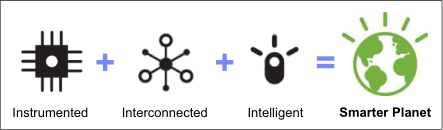
\includegraphics[width=0.7\linewidth]{figuras/pilares-da-iot}
    \caption{Os Três Pilares de um Planeta Inteligente}
    \label{fig:pilares-da-iot}
\end{figure}

A interconexão é construída pela conectividade com as redes locais e a
\textit{Internet} através de várias conexões física, tais como
\textit{Bluetooth}, \textit{Ethernet} e Fidelidade Sem Fio - \textit{Wireless
  Fidelity} (\textit{Wi-Fi}).

A instrumentação é construída pelos sensores e atuadores, no papel de
interfacear com o ambiente em indicar, monitorar e controlar os fenômenos de
diversas natureza. No processo de indicação estão os Diodos Emissores de Luz -
\textit{Light Emitting Diodes} (\textit{LEDs}) e os \textit{Displays}
Alfanumérico ou Gráfico. No processo de monitoração estão os sensores
eletrônicos para temperatura, umidade, presença, dentre outros... E no processo
de controle estão os motores e atuadores. Em uma constituição mais completa de
instrumentação estão a Identificação por Rádio Frequência -
\textit{Radio-Frequency IDentification} (\textit{RFID}), Sistema de
Posicionamento Global - \textit{Global Positioning System} (\textit{GPS}) e
Sistema de Navegação Inercial - \textit{Inertial Navigation System}
(\textit{INS}).

A inteligência é construída pelos algoritmos em \textit{software} embarcado, em
que realiza a junção do sistema computacional pelo processamento, análise e
ação da informação em conhecimento.

\section{Raspberry PI}

O \textit{Raspberry PI} é uma plataforma de desenvolvimento destinada para a
educação, desenvolvido por \textit{Even Upton} em 2006 da \textit{Raspberry PI
  Foundation}. A figura \ref{fig:raspberrypi} apresenta a versão
\textit{Raspberry PI B+} utilizada no objeto de estudo, um sistema baseado em
\textit{Linux} utilizando a arquitetura de Máquina \textit{RISC} Avançada -
\textit{Advanced RISC Machine} (\textit{ARM}) de baixo custo (por U\$ 40) do
tamanho de uma cartão de crédito.

\begin{figure}[H]
    \centering
    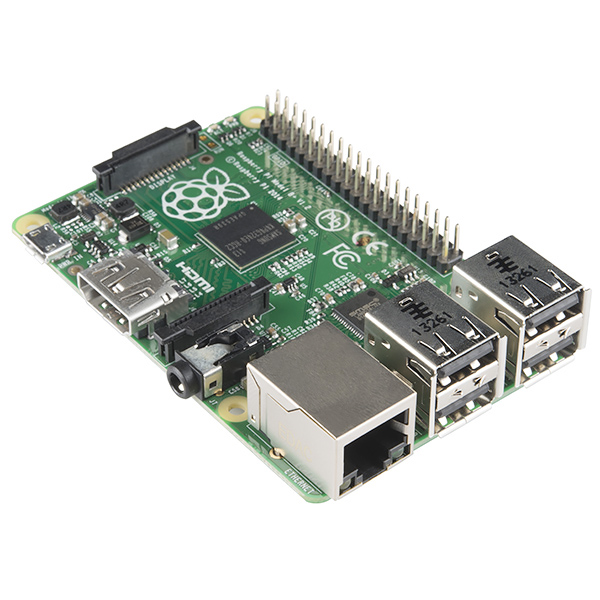
\includegraphics[width=10cm, height=10cm]{figuras/raspberrypi}
    \caption{Raspberry PI B+}
    \label{fig:raspberrypi}
\end{figure}

O ecossistema do \textit{Raspberry PI} possui uma grande comunidade na
\textit{Web}, diversas opções de \textit{hardware} periféricos, variações de
sistema operacionais \textit{Linux} como especializações para Tempo Real -
\textit{Real Time} (\textit{RT}) e Computador com um Conjunto Reduzido de
Instruções - \textit{Reduced Instruction Set Computer} (\textit{RISC}).

Existem outros sistemas para uso na \textit{Internet} das Coisas, tais como
\textit{BeagleBone}, \textit{Cubieboard}, \textit{Odroid} dentre outros... A
maioria baseada no mesmo sistema computacional do \textit{Raspberry PI}, com
sistema \textit{Linux} em arquitetura \textit{ARM}.

% ---
% CARACTERIZAÇÃO DO JAVA EMBEDDED
%
% ---

% TODO
% - revisão do texto em .pdf

\chapter{Caracterização do Java Embedded}

O \textit{Java Embedded} oferece aos desenvolvedores o estado da arte de uma
plataforma otimizada para um espectro de dispositivos embarcados, envolvendo
bibliotecas e ferramentas para o melhor aproveitamento dos Sistema-em-um-chip -
\textit{System-on-a-chip} (\textit{SoC}) através de um conjunto de plataformas,
conforme o \textit{footprint} da aplicação a ser desenvolvida.

A plataforma possui componentes 100\% em código \textit{Java}, desenvolvendo
aplicações embarcadas mais simples do que em plataforma \textit{C}, integrando
ferramentas de desenvolvimento, tais como \textit{NetBeans} e
\textit{Eclipse}. Os \textit{bytecodes} compilados para \textit{desktop} são
identicos aos executados no embarcado, com exceção da velocidade de execução,
permitindo as etapas de desevolvimento como codificação, execução,
\textit{debug} e \textit{profile} sem a necessidade do dispositivo embarcado.

\section{Plataforma Java Embedded}

As plataformas abordadas no respectivo trabalho serão: \textit{Java ME
  Embedded}, \textit{Java Embedded Suite} (\textit{JES}) e \textit{Java Oracle
  Event Processing} (\textit{OEP}).

\subsection{Java ME Embedded}

O \textit{Java ME Embedded} é uma versão reestruturada da plataforma
\textit{Java ME} com a inclusão da \textit{Device I/O API} (Entrada/Saída -
\textit{Input/Output}) (Interface de Programação de Aplicação -
\textit{Application Programming Interface}), destinadas aos periféricos de
baixo nível encontrados nos dispositivos embarcados, tais como Entrada/Saída de
Propósito Geral - \textit{General Purpose Input/Output} (\textit{GPIO}),
Conversor Analógico para Digital - \textit{Analog to Digital Converter}
(\textit{ADC}), Circuito Inter-Integrado - \textit{Inter-Integrated Circuit}
(\textit{I2C}), Interface Periférica Serial - \textit{Serial Peripheral
  Interface} (\textit{SPI}), Transmissor/Receptor Assíncrono Universal -
\textit{Universal Asynchronous Receiver/Transmitter} (\textit{UART}) e etc.

A plataforma \textit{Java ME Embedded} consiste de duas versões:

\begin{itemize}

    \item \textit{Java ME Embedded}: dedicado para as aplicações sempre ativa
    (\textit{always-on}), sem interface gráfica com o usuário
    (\textit{headless}) e com conexões a dispositivos. Possui
    \textit{footprint} menor que 1 \textit{megabyte} de memória;

    \item \textit{Java ME Embedded Client}: dedicado para as aplicações com
    maior necessidade de características da plataforma \textit{Java}. Possui
    \textit{footprint} menor que 10 \textit{megabytes} de memória.

\end{itemize}

Exemplos de aplicações:

\begin{itemize}

    \item prototipagem para aplicações de computação embarcada;

    \item possibilidades para utilização de sensores como fonte de dados em
    aplicações para o conceito \textit{Internet} das Coisas -
    \textit{Internet of Things} (\textit{IoT}).

\end{itemize}

\subsection{Java Embedded Suite}

O \textit{JES} é uma versão da plataforma \textit{Java EE} (Edição Empresarial
- \textit{Enterprise Edition}) para os sistemas embarcados, trazendo a
capacidade da arquitetura Cliente/Servidor - \textit{Client/Server} através de
banco de dados - \textit{databases}, serviços \textit{Web} - \textit{Web
  services} e aplicações \textit{Servlet}.

Os componentes disponíveis para a plataforma são:

\begin{itemize}

    \item \textit{GlassFish}: versão reduzida do servidor de aplicações
    \textit{GlassFish}, com suporte apenas para os componentes \textit{Servlet
    3.0} e \textit{Bean Validation 1.0};

    \item \textit{Java DB}: versão otimizada do banco de dados \textit{Derby}
    para uso embarcado (não possui características para arquitetura
    Cliente/Servidor), acessado via Linguagem de Consulta Estruturada -
    \textit{Structured Query Language} (\textit{SQL}) sobre o Conectividade de
    Banco de Dados \textit{Java} \textit{Java Database Connectivity}
    (\textit{JDBC});

    \item \textit{Jersey}: \textit{framework} para serviços \textit{RESTful Web
    Services}, conforme a especificação \textit{JAX-RS} (\textit{JSR 311}).

\end{itemize}

\subsection{Java Oracle Event Processing}

O \textit{OEP} é uma versão do sistema de Processamento de Eventos Complexos -
\textit{Complex Event Processing} (\textit{CEP}) para os sistemas embarcados,
trazendo a capacidade de transformar dados em informação para os dispositivos.

\section{Vantagens e Desvantagens}

A plataforma \textit{Java Embedded} possui vantagens e desvantagens em relação
a plataforma nativa (\textit{C}).

\newpage
\subsection{Vantagens}

\begin{itemize}

    \item Suporte a aplicações \textit{headless}: serviços executados em
    segundo plano;

    \item Segurança \textit{sandbox}: a máquina virtual constrói um ambiente de
    execução para a aplicação, diferentemente da plataforma nativa em que não
    possui a característica;

    \item Múltiplos processos: capacidade para execução multitarefa de
    aplicações;

    \item Comunidade: a tecnologia \textit{Java} possui uma grande comunidade
    de desenvolvedores em todo mundo, ideal para o aprendizado e suporte, na
    plataforma nativa a comunidade é fragmentada;

    \item Escalabilidade: excelente capacidade de gerenciamento de recursos e
    adição de novas funcionalidades a aplicação;

    \item Capacidade de atualização: a execução em máquina virtal traz para o
    sistema possui um excelente mecanismo para atualização da aplicação, na
    plataforma nativa o sistema é inferior em dificuldade.

\end{itemize}

\subsection{Desvantagens}

A principal desvantagem em relação a plataforma nativa está no desempenho, pois
a máquina virtual utiliza de recursos como memória e processamento, além dos
requeridos para a aplicação.

Uma abordagem para minimizar os problemas está em definir \textit{profiles}
para o tipo de aplicação, assim reduzindo a carga da máquina virtual.

\section{Otimização da JVM}

A Máquina Virtual Java - \textit{Java Virtual Machine} (\textit{JVM}) é
otimizada para as Unidades Central de Processamento - \textit{Central
  Processing Units} (\textit{CPU}) da arquitetura (\textit{ARM}), com suporte a
\textit{hard-float} no \textit{Kit} de Desenvolvimento \textit{Java} -
\textit{Java Development Kit} (\textit{JDK}) 1.8. Várias plataformas de
\textit{hardware} são compatíveis como: \textit{ARM}, \textit{Intel},
\textit{Atmel}, dentro outros.

% ---
% METODOLOGIA
%
% ---

\chapter{Metodologia}

A metodologia adotada para o objeto de estudo foca na observação da tecnologia
\textit{Java} para o desenvolvimento no conceito \textit{Internet} das Coisas -
\textit{Internet of Things} (\textit{IoT}) através de três diferentes escopos
de aplicações. A experimentação das aplicações proporcionará um amplo alcance
de possibilidades, por meio das bibliotecas e ferramentas de \textit{software}.

Os escopos selecionados para a experimentação são:

\begin{itemize}

    \item periféricos de baixo nível: apresentar as Interfaces de Programação
    de Aplicação - \textit{Application Programming Interfaces} (\textit{APIs})
    e periféricos destinados a comunicação e interfaceamento de baixo nível com
    o \textit{Raspberry PI}. A aplicação utilizará o \textit{Java ME} (Edição
    Micro - \textit{Micro Edition}) com a \textit{Device I/O API}
    (Entrada/Saída - \textit{Input/Output});

    \item arquitetura cliente/servidor: apresentar a utilização de servidores
    no \textit{Raspberry PI}. A aplicação utilizará o \textit{Java Embedded
        Suite} (\textit{JES});

    \item processamento de eventos complexos: apresentar o ambiente para
    desenvolvimento de Processamento de Eventos Complexos - \textit{Complex
        Event Processing} (\textit{CEP}).  A aplicação utilizará o \textit{Java
        Oracle Event Processing} (\textit{OEP}).

\end{itemize}

As aplicações serão desenvolvidas pelo Ambiente de Desenvolvimento Integrado -
\textit{Integrated Development Environment} (\textit{IDE}) \textit{Netbeans}
8.0.2 com o \textit{Kit} de Desenvolvimento de \textit{Software} -
\textit{Software Development Kit} (\textit{SDK}) \textit{Java} 8. O sistema
base é composto de um ambiente virtualizado no \textit{Oracle VM VirtualBox}
com o sistema operacional \textit{Linux Debian}. No caso do \textit{Java ME SDK
    8 Embedded} será utilizado através do sistema operacional \textit{Windows}
7, pois não há uma versão para o sistema operacional \textit{Linux}.

As aplicações serão testadas com a plataforma de prototipagem \textit{Raspberry
    PI B+} com o sistema operacional \textit{Raspbian - Debian Wheezy} versão
de 16/02/2015.

A comunicação do computador de desenvolvimento e a plataforma de prototipagem
será pelo acesso remoto com os utilitários \textit{Secure Shell} (\textit{SSH})
e \textit{Virtual Network Computing} (\textit{VNC}) por rede \textit{Ethernet}.

Os resultados serão apresentados através da indicação das principais vantagens
e desvantagem observadas, dentro do conceito \textit{IoT}.

% ---
% JAVA ME EMBEDDED
%
% ---

\chapter{Java ME Embedded}

Este capítulo tem como objetivo demonstrar a plataforma \textit{Java Embedded}
- \textit{Java ME Embedded}.

\section{Instalação}

A plataforma de prototipagem deve estar operacional com o sistema operacional
\textit{Linux} e a plataforma \textit{Java 8}, no caso de estudo a plataforma
\textit{Raspberry PI B+}. A figura \ref{fig:java-me/configuracao} apresenta as
configurações do sistema em estudo.

\begin{figure}[H]
    \centering
    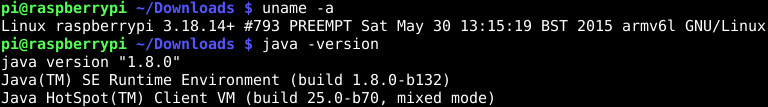
\includegraphics[width=0.7\linewidth]{figuras/java/configuracao}
    \caption{Configuração do Sistema}
    \label{fig:java-me/configuracao}
\end{figure}

Para a plataforma de prototipagem é necessário a instalação do pacote
\textit{Oracle Java ME Embedded 8.1 for Raspberry Pi Model B (ARM11/Linux)},
necessário ter uma conta no site da \textit{Oracle} para realizar o
\textit{download}.

Transfira o arquivo
\verb|oracle-jmee-8-1-rr-raspberrypi-linux-bin.zip| do sistema operacional
principal para o dispositivo remoto, basta utilizar o comando \textit{SCP}:

\verb|scp </path/from/file> <user>@<address>:/path/to/destination|

Descompacte o arquivo, basta utilizar o comando \textit{UNZIP}:

\verb|unzip <file>|

Aplique a permissão 777 para os diretórios \textit{appdb} e \textit{bin}, basta
utilizar o comando \textit{CHMOD}:

\verb|chmod -R 777 appdb bin|

\subsection{Pacote Oracle Java ME Embedded ZIP}

O pacote \textit{Oracle Java ME Embedded ZIP} consiste de cinco diretórios:

\begin{itemize}

    \item /appdb: este diretório é utilizado pela plataforma de prototipagem e
    contém as bibliotecas interna do \textit{Java};

    \item /bin: este diretório é utilizado pela plataforma de prototipagem para
    instalar, executar e remover as aplicações \textit{IMlets}, possui os
    executáveis, \textit{scripts} e o arquivo de configuração do
    \textit{Java} \verb|jwc_properties.ini|;

    \item /legal: este diretório contém a documentação de licença;

    \item /lib: este diretório é utilizado no processo de compilação dos
    \textit{IMlets}, contém os arquivos necessários para a execução do
    \textit{Developer Agent};

    \item /util: este diretório possui o arquivo \verb|proxy.jar|, requerido
    para a comunicação entre plataforma de prototipagem e \textit{Desktop}
    através do \textit{Developer Agent}.

\end{itemize}

No \textit{NetBeans IDE 8} ative o \textit{Java ME}, instale os arquivos
\textit{Oracle Java ME SDK 8.1} e \textit{plugin} \textit{Oracle Java ME SDK
  8.1 Plugins for NetBeans 8}, necessário ter uma conta no site da
\textit{Oracle} para realizar o \textit{download}. O \textit{Oracle Java ME SDK
  8.1} somente possui versão para o sistema operacional \textit{Windows
  x86/64}.

\subsection{Desenvolvimento}

O processo de desenvolvimento inicia pela codificação da aplicação, em seguida
seu aprimoramento pela documentação da Interfaces de Programação de Aplicação -
\textit{Application Programming Interfaces} (\textit{APIs}), quando concluído é
exercitado pelo emulador e finalmente a implantação no dispositivo.

O exemplo aplicado trata-se de um gerador de Modulação por Largura de Pulso -
\textit{Pulse-Width Modulation} (\textit{PWM}) para a produção de sinais para
fins como transmitir informações em baixo nível para outros dispositivos.

\subsubsection{Codificação}

A aplicação consiste de um \textit{software} \textit{IMlet}, uma classe na qual
estende \newline
 \verb|javax.microedition.midlet.MIDlet| e implementa dois métodos:

\begin{itemize}

    \item \verb|startApp()|: sinaliza a aplicação a transição para o estado
    Ativo.

    \item \verb|destroyApp()|: sinaliza a aplicação a transição para o estado
    Destruído.

\end{itemize}

O código final é apresentado abaixo:
\newpage
\begin{verbatim}
// JavaMEExample.java
package ufabc;

import java.io.IOException;
import javax.microedition.midlet.MIDlet;
import jdk.dio.DeviceManager;
import jdk.dio.pwm.PWMChannel;

public class JavaMEExample extends MIDlet {

    PWMChannel channel;

    @Override
    public void startApp() {
        System.out.println("Início da Aplicação");
        try {
            channel = (PWMChannel) DeviceManager.open(18);
            channel.setPulsePeriod(1000000);
            channel.generate(500000, 10);
        } catch (IOException ex) {
        }
    }

    @Override
    public void destroyApp(boolean unconditional) {
        try {
            channel.close();
        } catch (IOException ex) {
        }
        System.out.println("Encerramento da Aplicação");
    }
}
\end{verbatim}

O acesso aos periféricos são realizados através da permissão da \textit{API}
pela requisição do \verb|jdk.dio.DeviceMgmtPermission| em Descritor de
Aplicações - \textit{Application Descriptor}, a figura
\ref{fig:java-me/application-descriptor} apresenta as permissões para o exemplo
acima.

\begin{figure}[H]
    \centering
    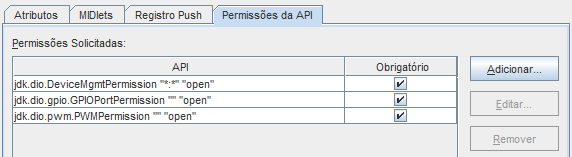
\includegraphics[width=0.7\linewidth]{figuras/java/java-me-application-descriptor.png}
    \caption{Descritor de Aplicações}
    \label{fig:java-me/application-descriptor}
\end{figure}

\subsubsection{Device I/O API}

A \textit{Device I/O API} (Entrada/Saída - \textit{Input/Output}) (Interface de
Programação de Aplicação - \textit{Application Programming Interface}) provê
uma biblioteca para o acesso aos periféricos de baixo nível em sistema
embarcados através da plataforma \textit{Java}. Sua utilização possui a mesma
simplicidade das demais bibliotecas do pacote \textit{Java}, pois basta a
consulta ao \textit{javadoc} e aplicar as implementações. A figura
\ref{fig:java-me/java-me-javadoc-deviceioapi} apresenta a estrutura
\textit{javadoc} dos pacotes do \textit{Device I/O API}.

\begin{figure}[H]
    \centering
    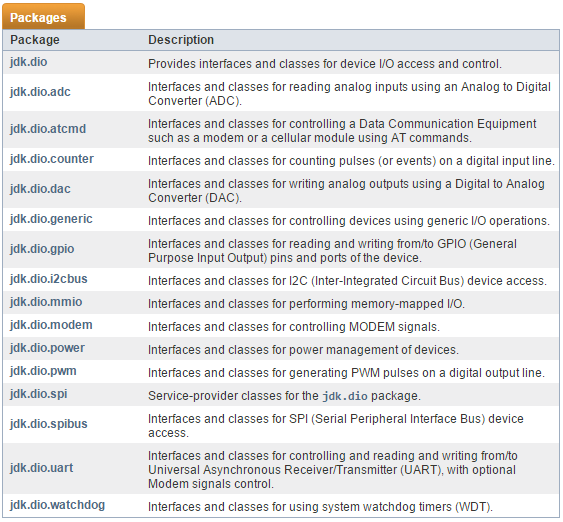
\includegraphics[width=0.7\linewidth]{figuras/java/java-me-javadoc-deviceioapi.png}
    \caption{Pacotes do Device I/O API}
    \label{fig:java-me/java-me-javadoc-deviceioapi}
\end{figure}

\subsubsection{Emulador}

O \textit{Java ME SDK 8 Embedded} incorpora uma emulador de dispositivos para a
visualização e controle dos periféricos e recursos encontrados nos
dispositivos, na figura \ref{fig:java-me/emulator} apresenta a tela inicial do
emulador e na figura \ref{fig:java-me/pwm} a visualização da execução do
aplicativo de \textit{PWM}.

\begin{figure}[H]
    \centering
    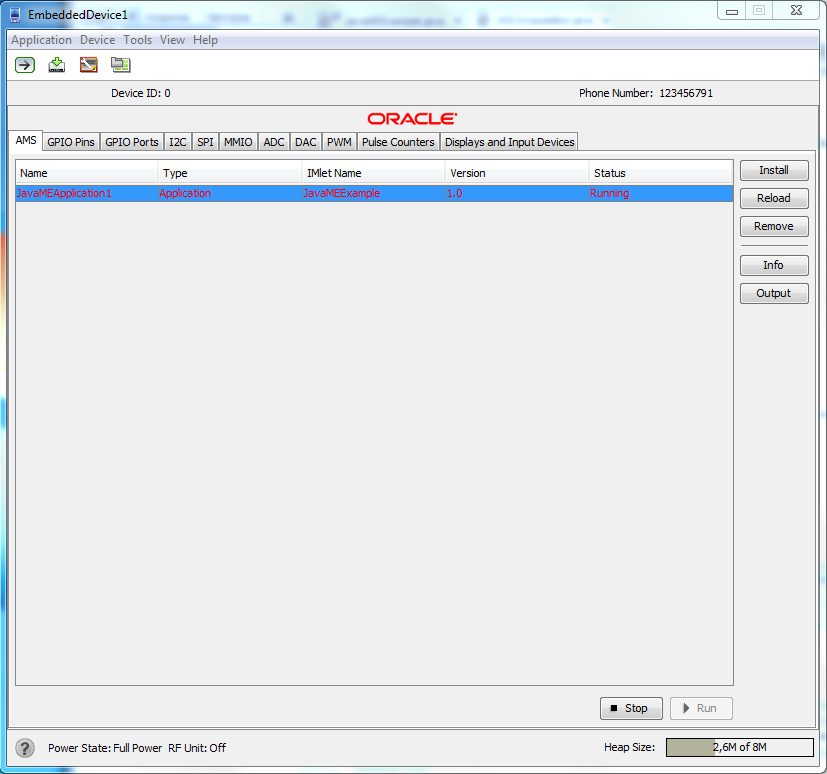
\includegraphics[width=0.7\linewidth]{figuras/java/java-me-emulator.png}
    \caption{Emulador}
    \label{fig:java-me/emulator}
\end{figure}

\begin{figure}[H]
    \centering
    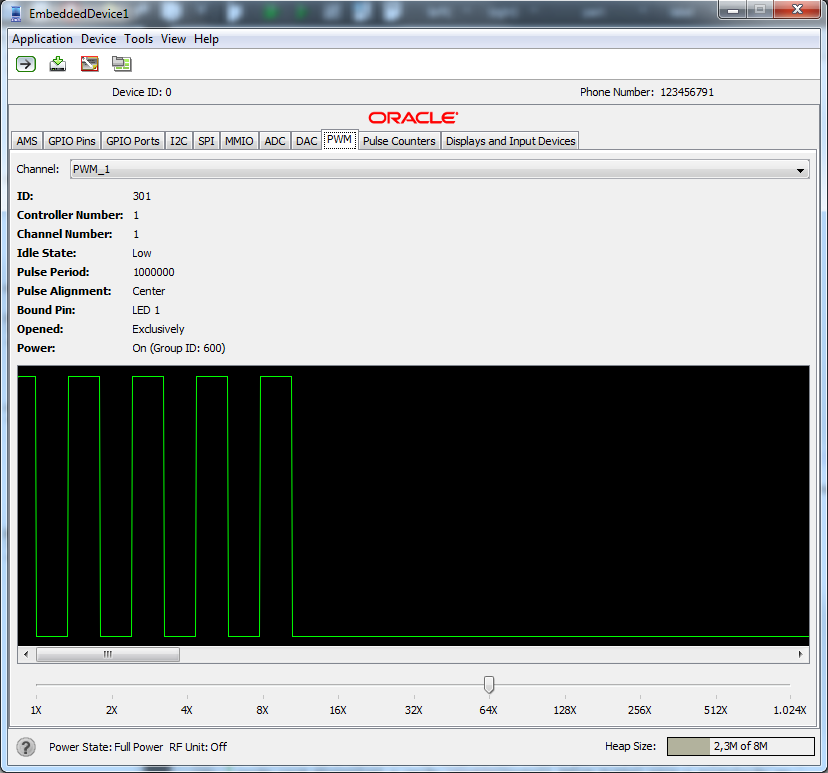
\includegraphics[width=0.7\linewidth]{figuras/java/java-me-pwm.png}
    \caption{Sinal PWM}
    \label{fig:java-me/pwm}
\end{figure}

Diversas ferramentas são encontradas no emulador, tais como controle de
conectividade, visualização da saída padrão e gerador de eventos externos, na
figura \ref{fig:java-me/external-events-generator} apresenta a tela para gerar
eventos para o periférico Entrada/Saída de Propósito Geral - \textit{General
  Purpose Input/Output} (\textit{GPIO}).

\begin{figure}[H]
    \centering
    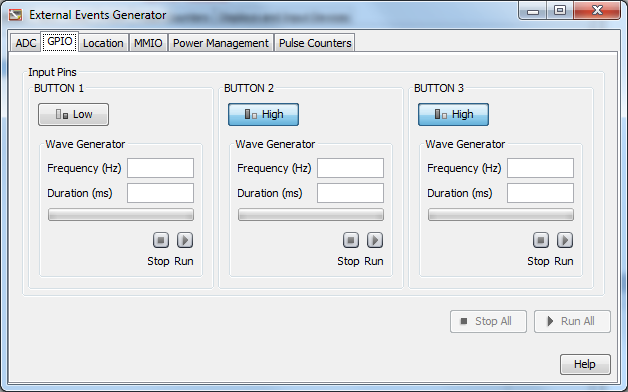
\includegraphics[width=0.7\linewidth]{figuras/java/java-me-external-events-generator.png}
    \caption{Emulador}
    \label{fig:java-me/external-events-generator}
\end{figure}

\subsubsection{Implantação}

O processo de implantação requer a execução do \textit{script}
\verb|usertest.sh| para a inicialização do \textit{Java} no dispositivo remoto.
No projeto escolha o dispositivo externo para a plataforma, como na figura
\ref{fig:java-me/plataform}.

\begin{figure}[H]
    \centering
    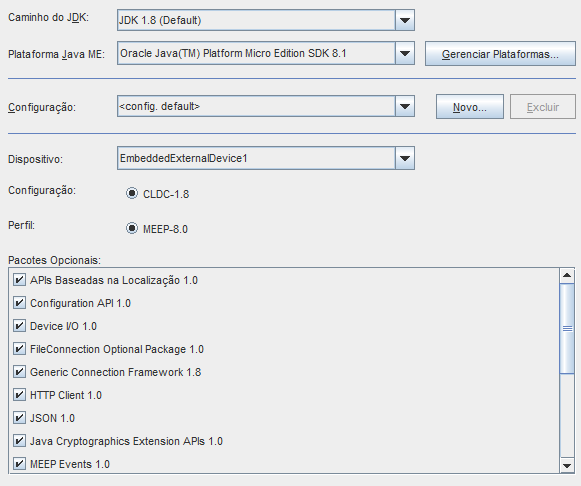
\includegraphics[width=0.7\linewidth]{figuras/java/java-me-plataform.png}
    \caption{Dispositivo Embarcado Externo}
    \label{fig:java-me/plataform}
\end{figure}

O emulador será conectado ao dispositivo remoto para a execução da aplicação,
porém será disponível a opção \textit{Install IMlet Suite} para a instalação no
dispositivo.

Outra opção é transferir a aplicação Descritor da Aplicação \textit{Java} -
\textit{Java Application Descriptor} (\textit{JAD}) para o dispositivo remoto e
executar o \textit{script} \verb|installMidlet.sh| e \verb|runSuite.sh|.

\section{Aplicações para a Internet das Coisas}

O interfaceamento com periféricos de baixo nível permite a utilização de uma
gama de fontes de dados, tais como sensores e atuadores. Esses dados podem
serem combinados com outros dispositivos embarcados.

\section{Resultados}

Os resultados demonstram a visão na qual a plataforma \textit{Java ME Embedded}
contribui para o desenvolvimento de aplicações destinadas a \textit{Internet}
das Coisas - \textit{Internet of Things} (\textit{IoT}).

\subsection{Positivos}

\begin{itemize}

    \item Permite uma abstração dos periféricos de baixo nível, sem a
    necessidade de endereços e estruturas de \textit{bits} através da
    \textit{Device I/O API};

    \item O Emulador auxilia no desenvolvimento de aplicações, por
    disponibilizar uma variedade de interfaces de \textit{hardware}.

\end{itemize}

\subsection{Negativos}

\begin{itemize}

    \item O \textit{Java ME 8 SDK} não possui uma versão para o sistema
    operacional \textit{Linux}, o que dificulta durante o ciclo de
    desenvolvimento;

    \item A aplicação necessidade ser inicializada pelo Sistema Operacional,
    para aplicações autônomas.

\end{itemize}

% ---
% JAVA EMBEDDED SUITE (JES)
%
% ---

\chapter{Java Embedded Suite}

Este capítulo tem como objetivo demonstrar a plataforma \textit{Java Embedded}
- \textit{Java Embedded Suite} (\textit{JES}).

\section{Instalação}

A plataforma de prototipagem deve estar operacional com o sistema operacional
\textit{Linux} e a plataforma \textit{Java 8}, no caso de estudo a plataforma
\textit{Raspberry PI B+}. A figura \ref{fig:jes/configuracao} apresenta as
configurações do sistema em estudo.

\begin{figure}[H]
    \centering
    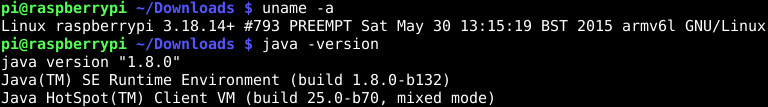
\includegraphics[width=0.7\linewidth]{figuras/java/configuracao}
    \caption{Configuração do Sistema}
    \label{fig:jes/configuracao}
\end{figure}

Para a plataforma de prototipagem é necessário a instalação do pacote
\textit{Oracle Java Embedded Suite 7.0}, necessário ter uma conta no site da
\textit{Oracle} para realizar o \textit{download}.

Transfira os arquivos \newline
\verb|jes-7.0-ga-bin-b11-linux-arm-runtime-15_nov_2012.zip|
 e \newline
\verb|jes-7.0-ga-b11-linux-samples-15_nov_2012.zip|
 do sistema operacional principal para o dispositivo remoto, basta
utilizar o comando \textit{SCP}:

\verb|scp </path/from/file> <user>@<address>:/path/to/destination|

Descompacte os arquivos, basta utilizar o comando \textit{UNZIP}:

\verb|unzip <file>|

O caminho para o \textit{JES} define a variável ambiente
\verb|$JES_HOME| no sistema. Os \textit{scripts} já definem as variáveis de
ambiente necessárias para o sistema executar cada tipo de aplicação do pacote
\textit{JES}.

\subsection{Pacote Oracle Java Embedded Suite ZIP}

O pacote \textit{Oracle Java Embedded Suite ZIP} consiste de cinco diretórios:

\begin{itemize}

    \item \textit{glassfish}: este diretório contém servidor de aplicações
    \textit{GlashFish} através da biblioteca \verb|glassfish-jes.jar|;

    \item \textit{javadb}: este diretório contém o banco de dados
    \textit{Derby} através das bibliotecas \verb|derby.jar| e
    \verb|derbytools.jar|;

    \item \textit{jersey}: este diretório contém o \textit{framework} de
    aplicações \textit{Jersey};

    \item \textit{jre}: este diretório contém o \textit{runtime} para a
    execução de aplicações \textit{Java}. Não é necessário, quando o
    \textit{Java 8} encontrasse corretamente instalado;

    \item \textit{samples}: este diretório contém exemplos de aplicações e os
    \textit{scripts} para a execução das aplicações.

\end{itemize}

O arquivo \verb|jes-verify.sh| realiza o diagnóstico da instalação do ambiente
de execução.

\subsection{Desenvolvimento}

O processo de desenvolvimento não difere da forma utilizada em servidores
tradicionais através de aplicações \textit{Web application}, em codificar e
realizar a implantação da aplicação.

O exemplo implementa uma aplicação \textit{Web} para a monitoração de
temperatura da Unidade de Processamento Gráfico - \textit{Graphics Processing
  Unit} (\textit{GPU}) do \textit{Raspberry PI} através do comando
\verb|/opt/vc/bin/vcgencmd measure_temp| do sistema operacional.

\subsubsection{Codificação}

A aplicação consiste de um \textit{software} \textit{Servlet} com a definição
do método \verb|doGet()|, sendo o código final apresentado abaixo:

\begin{verbatim}
// MonitorTemp.java
package ufabc;

import java.io.BufferedReader;
import java.io.IOException;
import java.io.InputStreamReader;
import javax.servlet.ServletException;
import javax.servlet.annotation.WebServlet;
import javax.servlet.http.HttpServlet;
import javax.servlet.http.HttpServletRequest;
import javax.servlet.http.HttpServletResponse;

@WebServlet(urlPatterns = {"/"})
public class MonitorTemp extends HttpServlet {

    @Override
    protected void doGet(HttpServletRequest request,
            HttpServletResponse response)
            throws ServletException, IOException {
        response.getWriter().write("<b>Monitoração da GPU<b><br/>");
        Runtime runtime = Runtime.getRuntime();
        BufferedReader br = new BufferedReader(
                new InputStreamReader(
                        runtime.exec("/opt/vc/bin/vcgencmd measure_temp")
                        .getInputStream()));
        response.getWriter().write(br.readLine());
    }
}
\end{verbatim}

\subsubsection{Implantação}

A implantação da aplicação é por transferir o arquivo para o dispositivo remoto
e executar via o \textit{script} para o tipo de aplicação:

\begin{itemize}

    \item \verb|gfhost.sh|: utilizado para implantar a aplicação \textit{Web}
    no \textit{JES}, permite múltiplas aplicações ao mesmo tempo;

    \item \verb|hclient.sh|: utilizado para acessar serviços \textit{Web} -
    \textit{Web services};

    \item \verb|hstorage.sh|: utilizado para aplicação com o \textit{Java DB};

    \item \verb|lwhost.sh|: utilizado para implantar a aplicação de serviço
      \textit{Web} no \textit{JES}.

\end{itemize}

O \textit{script} \verb|config.sh| permite a configuração do \textit{classpath}
e dos argumentos passados para o \textit{runtime} do \textit{Java}.

Para realizar a implantação do exemplo, basta utilizar o \textit{script}
\verb|gfhost.sh| no caminho \verb|$JES_HOME/samples/dist/run|:

\verb|./gfhost.sh ../../../dist/MonitorTemp.war|

Ao final da implantação será exibida a mensagem apresentada na figura
\ref{fig:java-me/java-jes-deploy}.

\begin{figure}[H]
    \centering
    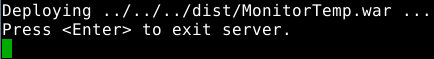
\includegraphics[width=0.7\linewidth]{figuras/java/java-jes-deploy.png}
    \caption{Implantação da Aplicação}
    \label{fig:java-me/java-jes-deploy}
\end{figure}

No navegador basta acessar o endereço do \textit{Raspberry PI} pela porta
\verb|8080| e adicionar o caminho da aplicação, conforme apresentado na figura
\ref{fig:java-me/java-jes-browser}.

\begin{figure}[H]
    \centering
    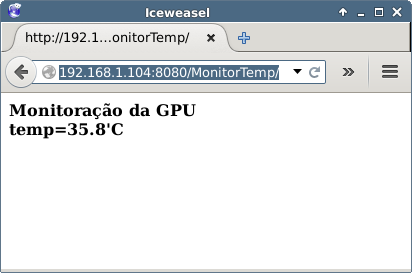
\includegraphics[width=0.7\linewidth]{figuras/java/java-jes-browser.png}
    \caption{Monitor de Temperatura da GPU}
    \label{fig:java-me/java-jes-browser}
\end{figure}

\section{Aplicações para a Internet das Coisas}

Um servidor de aplicações traz a \textit{Internet} das Coisas -
\textit{Internet of Things} (\textit{IoT}) uma interface para a
disponibilização de serviços, seja para a comunicação com usuários quanto
outros dispositivos embarcados. O \textit{JES} permite a interoperabilidade com
aplicações \textit{Java ME Embedded}, trazendo o poder dos periféricos de baixo
nível como fonte de dados. Esses serviços agrega as possibilidades de obtenção,
armazenamento e processamento de dados.

\newpage
\section{Resultados}

Os resultados demonstram a visão na qual a plataforma \textit{JES} contribui
para o desenvolvimento de aplicações destinadas a \textit{IoT}.

\subsection{Positivos}

\begin{itemize}

    \item A possibilidade de implantar um servidor de aplicações \textit{Web},
    banco de dados e serviços \textit{Web} em um sistema embarcado;

    \item Interfaceamento com as classes de aplicações \textit{Java ME
    Embedded}.

\end{itemize}

\subsection{Negativos}

\begin{itemize}

    \item Não possui muitos componentes para os servidores, assim reduzindo as
    possibilidades de desenvolvimento.

\end{itemize}

% ---
% JAVA ORACLE EVENT PROCESSING (OEP)
%
% ---

\chapter{Java Oracle Event Processing}

Este capítulo tem como objetivo demonstrar a plataforma \textit{Java Embedded}
- \textit{Java Oracle Event Processing} (\textit{OEP}).

\section{Instalação}

A plataforma de prototipagem deve estar operacional com o sistema operacional
\textit{Linux} e a plataforma \textit{Java 8}, no caso de estudo a plataforma
\textit{Raspberry PI B+}. A figura \ref{fig:oep/configuracao} apresenta as
configurações do sistema em estudo.

\begin{figure}[H]
    \centering
    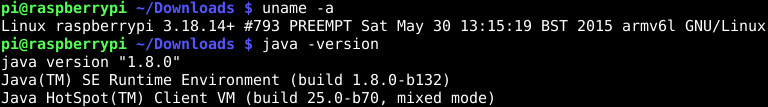
\includegraphics[width=0.7\linewidth]{figuras/java/configuracao}
    \caption{Configuração do Sistema}
    \label{fig:oep/configuracao}
\end{figure}

Para a plataforma de prototipagem é necessário a instalação do pacote
\textit{Oracle Java Embedded Suite 7.0} e \textit{Oracle Event Processing for
    Oracle Java Embedded}, necessário ter uma conta no site da \textit{Oracle}
para realizar o \textit{download}.

Transfira os arquivos \newline
\verb|jes-7.0-ga-bin-b11-linux-arm-runtime-15_nov_2012.zip|
, \newline
\verb|jes-7.0-ga-b11-linux-samples-15_nov_2012.zip|
e \newline
\verb|ofm_oep_embedded_11_1_1_7_1_linux.zip|
 do sistema operacional principal para o dispositivo remoto, basta utilizar o
comando \textit{SCP}:

\verb|scp </path/from/file> <user>@<address>:/path/to/destination|

Descompacte os arquivos, basta utilizar o comando \textit{UNZIP}:

\verb|unzip <file>|

\section{Aplicações para a Internet das Coisas}

O \textit{OEP} permite as aplicações na \textit{Internet} das Coisas -
\textit{Internet of Things} (\textit{IoT}), o processamento em tempo real dos
dados amostrados através dos periféricos e recursos encontrados nos
dispositivos, assim aplicando técnicas de filtragens e estatísticas para a
realização de análises.

\section{Resultados}

Os resultados demonstram a visão na qual a plataforma \textit{OEP} contribui
para o desenvolvimento de aplicações destinadas a \textit{IoT}.

\subsection{Positivos}

\begin{itemize}

    \item Grande poder de processamento, por oferecer uma gama de recursos para
    trabalhar com dados;

    \item Utilização de linguagem de consulta para a manipulação e amostragem
    dos dados;

    \item Traz a capacidade de \textit{gateway} para o dispositivo, quando
    conectado em outros dispositivos.

\end{itemize}

\subsection{Negativos}

\begin{itemize}

    \item Não possui uma interface de desenvolvimento produtiva como encontrada
    na versão tradicional através de linguagem gráfica.

\end{itemize}

% ---
% ANÁLISE DOS RESULTADOS
%
% ---

% TODO
% - incluir os resultados do OEP
% - revisão do texto em .pdf

\chapter{Análise dos Resultados}

O \textit{Java Embedded} é composto de diversos módulos para o desenvolvimento
de \textit{software} embarcado, compatível com as necessidades encontradas no
conceito de \textit{Internet} das Coisas - \textit{Internet of Things}
(\textit{IoT}).

No \textit{Java ME Embedded} são encontradas diversas ferramentas para o
desenvolvimento, juntamente com uma rica documentação do \textit{Device I/O
  API} (Entrada/Saída - \textit{Input/Output}) (Interface de Programação de
Aplicação - \textit{Application Programming Interface}). Entretanto a
plataforma não é fixa em apenas um sistema operacional, pois existem recursos
voltados para \textit{Windows} e outros para \textit{Linux}. A parte embarcada
é disponibilizada por uma estrutura de projeto com diversos \textit{scripts}
para a execução e/ou interfaceamento com o sistema operacional da aplicação
desenvolvida.

No \textit{Java Embedded Suite} (\textit{JES}) são disponibilizadas os
principais módulos para aplicações com servidores através de versões reduzidas
e otimizadas para o ambiente embarcado, no conceito \textit{IoT} faz uso de
tais aplicações por conectividade com outros sistemas e usuários. A plataforma
possui interoperabilidade com demais plataformas do \textit{Java Embedded},
trazendo um grande escopo de fonte de dados. O desenvolvimento é compatível com
o tradicional no Java EE (Edição Empresarial - \textit{Enterprise Edition}),
utilizando um número menor de componentes e sua implantação através de
\textit{scripts}, como no \textit{Java ME Embedded} com a vantagem do
interfaceamento com o sistema operacional.


% ---
% CONCLUSÃO
%
% ---

% TODO
% - refatorar os <tab> por <spaces> e wrap do texto, utilizando emacs
% - aplicar revisão do orientador
% - revisão do texto em .pdf

\chapter{Conclusão}

O conceito \textit{Internet} das Coisas alcança cada vez mais as aplicações do
dia a dia, trazendo novas possibilidades e desafios para o mundo da tecnologia.
A tecnologia \textit{Java} incorpora diversas ferramentas para o
desenvolvimento de sistemas embarcados através da plataforma \textit{Java
  Embedded}.

Diversos escopos são preenchidos, de periféricos de baixo nível até
processamento de eventos complexos, porém prover a característica de
produtividade não é o único ponto de escolha, o desempenho ainda é a principal
qualidade visada principalmente em dispositivos com baixo poder computacional.
O Java permite o meio termo entre desempenho e produtividade, principalmente
pela diversidade de ferramentas e Interfaces de Programação de Aplicação -
\textit{Application Programming Interfaces} (\textit{APIs}), como também
versões otimizadas da Máquina Virtual Java - \textit{Java Virtual Machine}
(\textit{JVM}).

Aspectos importantes a serem previstos estão na especificação e desenvolvimento
de protocolos, \textit{frameworks} e sistemas operacionais especializados.


% ---

% ----------------------------------------------------------
% ELEMENTOS PÓS-TEXTUAIS
% ----------------------------------------------------------
%\postextual
\nocite{reginaborgesdearaujo}
\nocite{francisdacosta2013}
\nocite{mcewencassimally2013}
\nocite{mqttibm2012}
\nocite{bahgamadisetti2014}
\nocite{tanenbaum2013structured}
\nocite{patterson2013computer}
\nocite{mateusloureiro2004}
\bibliography{bibliografia}

% ---

\end{document}
